\chapter{Concept}
\label{Concept}
The selection of navigation stacks is quite sparse. Especially considering the defined requirements. In general when it comes to navigation there are only two well documented stacks to choose from.

\begin{itemize}
	\item navigation\_stack
	\item MoveIt
\end{itemize}

In contrast to the navigation\_stack MoveIt is largely used for the path planning and navigation of industrial robot arms and therefore not suited for this application.

The navigation\_stack provides a general setup proposal which seems to be a good starting point for robot navigation, but it has multiple parts that will be modified to adhere to the defined requirements, that will be discussed in the following part.\\\\

\begin{figure}
	\begin{center}
		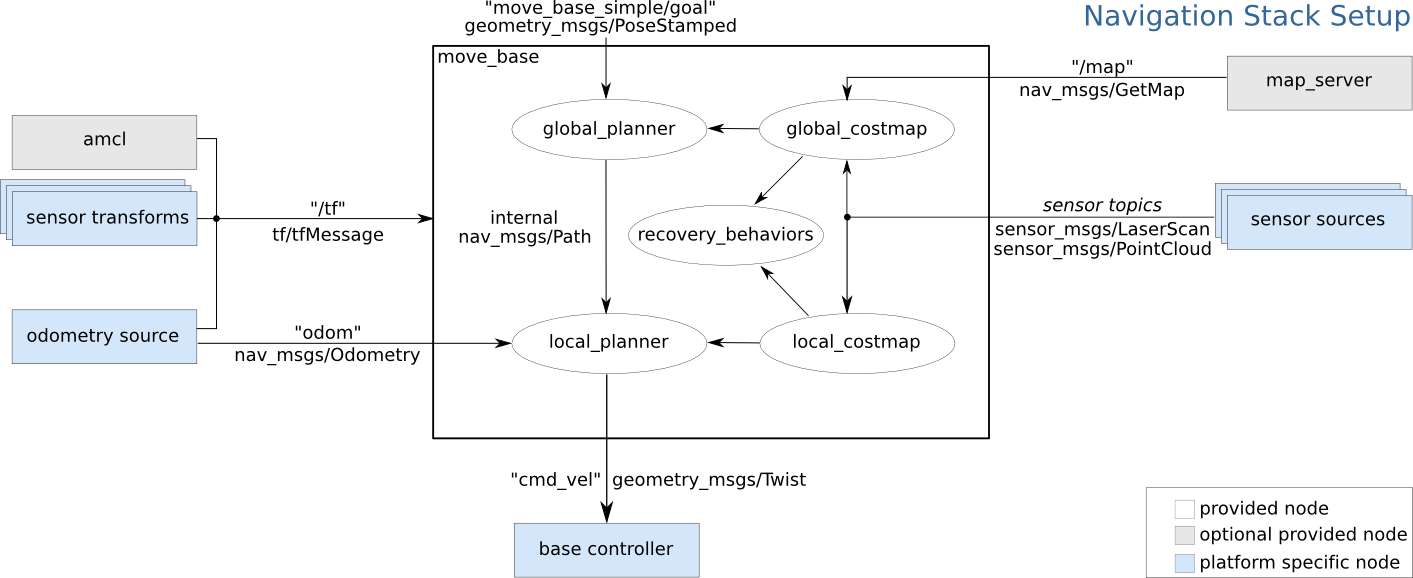
\includegraphics[width=140mm]{Pictures/navigation stack setup}
		\caption[navigation stack setup]{navigation stack setup}
	\end{center}
\end{figure}




\section{platform specific nodes}
Since the platform specific nodes are unique to each robot these will need to be adjusted.\\
\subsection{sensor sources}

The following sensors will be predefined for this concept:

\begin{itemize}
	\item lidar
	\item wheel encoder
	\item imu
	\item camera
\end{itemize}

Since these sensors will certainly have noise we firstly need to add additional filters for the sensor signals. 



\subsection{Odometry source}
The odometry is all ways a result of sensor data. Therefore we can make a direct connection between the sensor filters and the odometry input. These Filters will also feature nodes that transform the incoming sensor data into a useable format.

\subsection{Sensor transforms}
To know the position of every sensor relative to the robot and his odometry the tf\_tree has to be build. While this can be realised using static transform publishers there is also a cleaner way using the ros package robot\_state\_publisher. It then requires a robot description in URDF format that specifies the relations between everything mounted on the robot.
The transformation between the base of the robot and the odom will be build by the filtered odometry.

The remaining platform specific nodes are all available since the simulated robot will be used and provides a motor controller, as well as all of the sensors and data sources.

\section{Optional nodes}

The Map is a representation of the robots environment. If this is known from the start it is known, where the robot can go and where not.\\
 In this scenario the robot will always start blind, meaning it will not know anything about its surrounding other than that it can expect a road to be there, which makes the map\_server of the navigation\_stack and its functionality to convert prerecorded maps redundant.\\
Adding to that amcl (the localization package of the navigation\_stack) will no longer work since it tries to find a position in a predefined map based on the current sensor signals.\\
Knowing the environment and the position of the robot in it is an important part in robot navigation since it allows to send goals that are relative to the environment and not to the robot. That is why the usage of a SLAM algorithm becomes highly useful. This node supplies both the current map and the position of the robot in it.\\
This node will publish the transform between the map and the odom frame so the position of the robot and every sensor signal can be determined relative to the map frame.\\

\section{Provided nodes}

The provided nodes do not have to be reordered but the recovery behaviors will be removed. These will be incorporated in the incoming goals instead.

\section{PoseFinder}
The job of this node is to extract the pose of a goal from the sensor data or the map (if available).\\

The requirements of this node will be defined in the "Configuration and testing" section

\section{Resulting concept}
The following simplified schematic is the concept of the navigation stack setup. Not all of the connections between the nodes will be highlighted, to make the schematic easier to understand.\\

\begin{figure}
	\begin{center}
		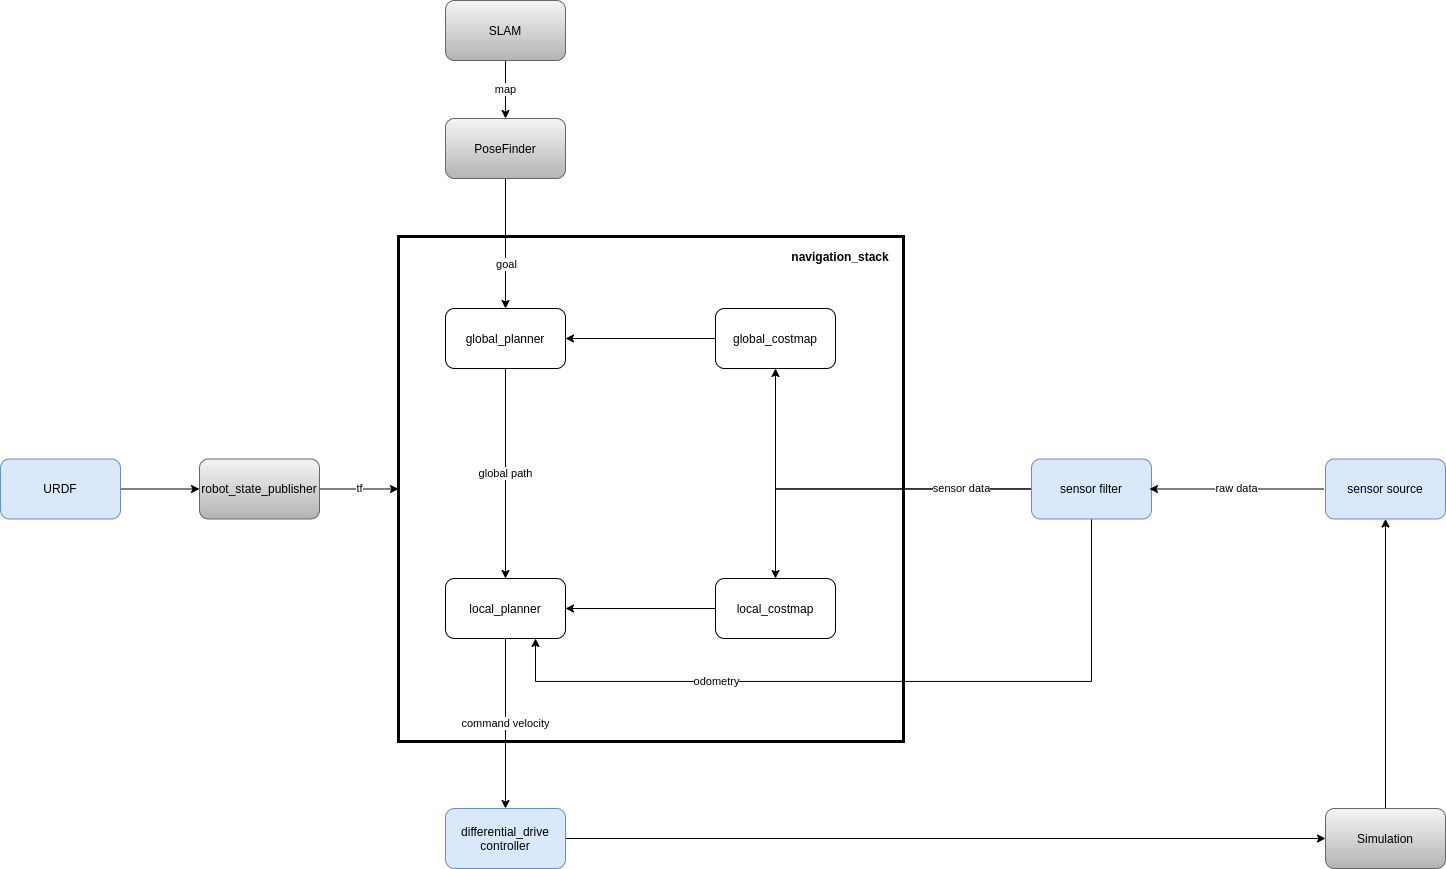
\includegraphics[width=140mm]{Pictures/Updated navigation concept}
		\caption[Updated navigation concept]{Updated navigation concept}
	\end{center}
\end{figure}



The PoseFinder will first find a goal based on the current state of the map and the sensor data and sends it to the navigation stack. This then uses the filtered sensor data to determine, where the robot is, where it is allowed to go and where not. The cascading planners then determine first a rough, collision free, path and then a path that is possible for the kinematics of the robot. This path will be send to the motor controller of the simulated robot.\\
This procedure will be repeated at a configurable frequency so the robot will never reach its finish. This is necessary since it is unknown if the goal, in the space that has not been explored yet, is perfectly on the future road, or if it is in an obstacle.




